%En la figura \ref{fig:infoProfesores} se puede observar la información que el \refElem{Calmecac} utilizará de acuerdo a los servicios web proporcionados por el \refElem{SIEE}.%Verificar
%
%\begin{figure}[hbtp!]
%	\begin{center}
%	\fbox{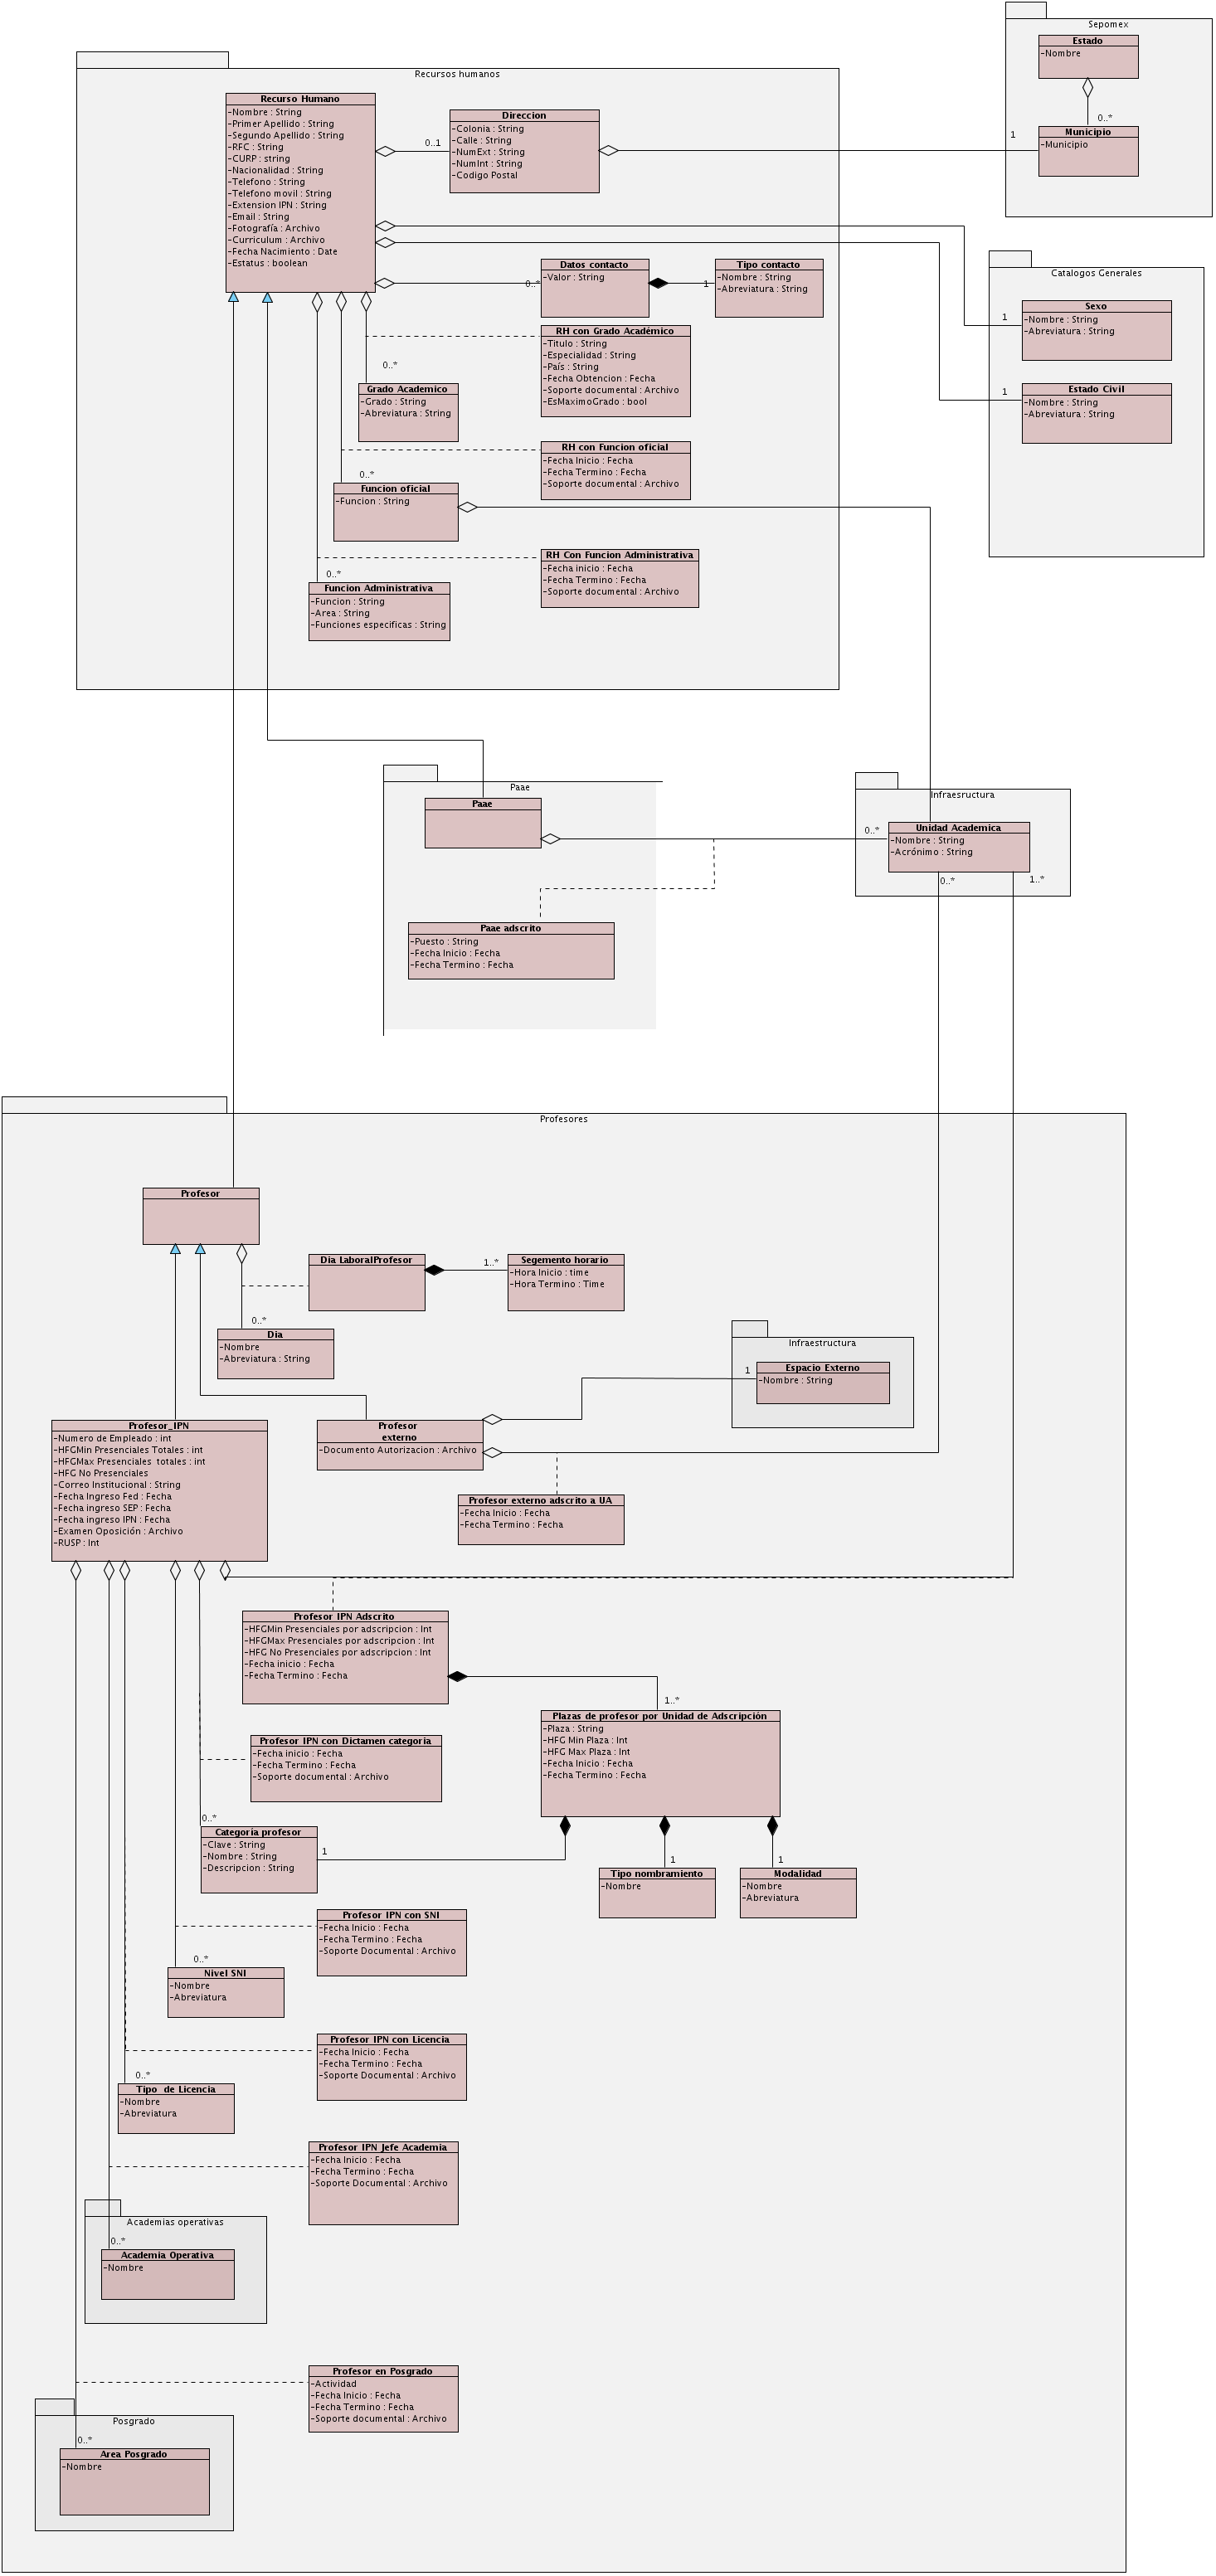
\includegraphics[width=\textwidth]{negocio/images/ModeloDeInformacion_Profesores}}
%		\label{fig:infoProfesores}
%		\caption{Modelo de Información de Profesores}
%	\end{center}
%\end{figure}

%===================================Paquete RECURSOS Humanos
%----------------------------------Recurso Humano--------------------------------------
\begin{cdtEntidad}[Es una persona que forma parte del Instituto Politécnico Nacional y que se encarga de realizar actividades administrativas y de gestión en las Unidades Académicas, Unidades Administrativas, Centros de Investigación o en los Órganos Consultivos. Su relación con el Instituto puede estar determinada por un contrato o por un convenio con una Unidad de Adscripción en específico.]{RecursoHumano}{Recurso Humano}
	\brAttr{nombre}{Nombre}{frase}{Representa la palabra o conjunto de palabras con las que se designan y se distinguen a una persona que labora en el Instituto.}{\datRequerido}
	\brAttr{primerApellido}{Primer apellido}{frase}{Representa la palabra o conjunto de palabras que sigue al nombre de pila de una persona y que se transmite de padres a hijos.}{\datRequerido}
	\brAttr{segundoApellido}{Segundo apellido}{frase}{Representa la palabra o conjunto de palabras que sigue al primer apellido de una persona y que se transmite de padres a hijos.}{\datOpcional}
	\brAttr{RFC}{RFC}{palabra}{Representa la clave alfanumérica compuesta de 13 caracteres que permite cumplir con las obligaciones que la ley establece para el pago de impuestos. En el Instituto es un mecanismo que ayuda a identificar a una persona que labora o apoya en las actividades académicas y administrativas. }{\datRequerido}
	\brAttr{CURP}{CURP}{palabra}{Representa la clave alfanumérica compuesta de 18 caracteres que permite identificar a un ciudadano residente de México. En el Instituto es otro de los mecanismos que ayudan a identificar a una persona que labora o apoya en las actividades académicas y administrativas.}{\datRequerido}
	\brAttr{fechaDeNacimiento}{Fecha de Nacimiento}{fecha}{Es la fecha que, en el Acta de Nacimiento de una persona, establece el día en que nació.}{\datRequerido}
	\brAttr{fechaDeUltimaActualizacion}{Fecha de última actualización}{fecha}{Indica la fecha en la que en el sistema se llevo a cabo una modificación o actualización en los datos o relaciones de una persona con otras entidades.}{\datOpcional}
	\brAttr{numeroDeEmpleado}{Número de Empleado}{entero}{Secuencia de dígitos numéricos que se utiliza para identificar a un profesor contratado por la Dirección Capital Humano. Su expresión regular es : $ [0-9]\{6,\}$. Este número no le es otorgado al personas que es contratado por honorarios o como visitante.}{\datOpcional}
	\brAttr{Activo}{Activo}{booleano}{Dato que representa si un recurso humano del Instituto se encuentra: \begin{Citemize}
			\item Activo -- Indica que el Recurso Humano se encuentra realizando actividades académicas y/o administrativas en el momento de su consulta.
			\item Inactivo -- Indica que el Recuro Humano no se encuentra realizando actividades académicas y/o administrativas en el momento de su consulta.
	\end{Citemize}}{\datOpcional}
	\brAttr{sexo}{Sexo}{Sexo}{Indica la sexualidad de un recurso humano con base en su acta de nacimiento.}{\datOpcional}
	\brAttr{pais}{País}{Pais}{Indica la nacionalidad de un recurso humano y que indica su relación con un país por medio de un gentilicio.}{\datOpcional}
	\cdtEntityRelSection
	\brRel{\brRelAgregation}{\refElem{tdGradoAcademico}}{Un Recurso Humano ha adquirido una o varias distinciones académicas a lo largo de su vida que ayudan a determinar, en algunos casos su categoría o posición dentro del Instituto así como su asignación de exposiciones para impartir los contenidos de una o varias Unidades de Aprendizaje.}
	\brRel{\brRelComposition}{\refElem{Documento}}{Un Recurso Humano adquiere una o más pruebas materiales que acreditan un grado, logro académico o algún otro documento en donde se establezca un aspecto relevante para la asignación de labores.}
	\brRel{\brRelComposition}{\refElem{ContactoDeRecursoHumano}}{Un Recurso Humano tiene uno o varios medios de contacto que se pueden utilizar para comunicarse con el o para enviarle notificaciones.}
	\brRel{\brRelAgregation}{\refElem{UnidadDeAdscripcion}}{Un Recurso Humano puede estar asignado a más de una Unidad de Adscripción en donde desempeña las labores designadas por un contrato o por un convenio.}
	\brRel{\brRelGeneralization}{\refElem{ProfesorIPN}}{Un Profesor que labore en el Instituto es un Recurso Humano que es considerado para la designación de labores docentes y de investigación en una o más unidades de adscripción.}
\end{cdtEntidad}

\begin{cdtEntidad}[Es uno de los métodos con los que se cuenta para comunicarse o ubicar a una persona y mantenerle informado acerca de noticias, notificaciones y cambios en los distintos procesos del Instituto que así lo requieran.]{ContactoDeRecursoHumano}{Contacto de Recurso Humano}
	%=======Atributos
	\brAttr{contacto}{Contacto}{palabra}{Es el conjunto de caracteres que representan a un mecanismo que se utiliza para poder comunicarse con un recurso humano.}{\datRequerido}
	\brAttr{contactoAuxiliarA}{Contacto Auxiliar A}{palabra}{Es un carácter o conjunto de caractere que tienen la utilidad de almacenar información adicional.}{\datOpcional}
	\brAttr{contactoAuxiliarB}{Contacto Auxiliar B}{palabra}{Es un carácter o conjunto de caractere que tienen la utilidad de almacenar información adicional.}{\datOpcional}
	\brAttr{tipoDeContacto}{Tipo de Contacto}{TipoDeContacto}{Se utiliza para especificar y clasificar al contacto por sus características.}{\datRequerido}
	%======Relaciones
	\cdtEntityRelSection
	\brRel{\brRelComposition}{\refElem{RecursoHumano}}{Un recurso humano tiene uno o varios medios de contacto que se pueden utilizar para comunicarse con el o para enviarle notificaciones.}
\end{cdtEntidad}

%---------------------------------------RHGrado Académico--------------------------------------------%
\begin{cdtEntidad}[En es el resultado de la relación entre \refElem{RecursoHumano} y \refElem{tdGradoAcademico} y tiene como propósito almacenar todas aquellas distinciones académicas que un Recurso Humano ha adquirido con el paso de tiempo y que se utiliza como apoyo al definir la asignación de exposiciones de Unidades de Aprendizaje a Grupos.]{RecursoHumanoConGradoAcademico}{Recurso Humano con Grado Académico}
	%====Atributos
	\brAttr{titulo}{Titulo}{frase}{Conjunto de palabras que representan un grado y el programa de estudios  adquirido por un recurso humano.}{\datRequerido}
	\brAttr{fechaDeObtencion}{Fecha de Obtención}{fecha}{Indica el día en que un grado académico se adquiere. Está fecha puede encontrarse en el documento que avala la adquisición de un grado del Recurso Humano.}{\datRequerido}	
	\brAttr{fechaDeExpedicion}{Fecha de Expedición}{fecha}{Indica el día en que el documento que avala la adquisición de un grado es emitido.}{\datOpcional}	
	\brAttr{esUltimoGrado}{Es Último Grado}{booleano}{Indica si el grado adquirido es el máximo obtenido por el \refElem{RecursoHumano} tomando como referencia otras distinciones adquiridas, si las tiene, o en la escala del nivel educativo correspondiente.}{\datRequerido}	
	\brAttr{pais}{País}{Pais}{Indica el país de procedencia del grado obtenido por el recurso humano.}{\datRequerido}	
	\brAttr[Entidad]{documento}{Documento}{Documento}{Un grado académico adquirido por un recurso humano es avalado por una prueba material en el que se especifica la conclusión de un programa de estudios. }{\datRequerido}
\end{cdtEntidad}

\begin{cdtEntidad}[Es la prueba material que contiene información acerca de un hecho académico o laboral de un Recurso Humano y que es emitida por instituciones o personas físicas o morales.]{Documento}{Documento}
	\brAttr{nombre}{Nombre}{frase}{Es la palabra o el conjunto de palabras que tienen como propósito identificar una prueba material que contiene información acerca de un hecho académico o laboral de un Recurso Humano.}{\datRequerido}		
	\brAttr{fechaDeInicio}{Fecha de Inicio}{fecha}{Indica el día en que inicia la validez de una prueba material que sirve para especificar un nombramiento, un logro académico o una actividad.}{\datRequerido}
	\brAttr{fechaDeFin}{Fecha de Fin}{fecha}{Indica el día en que concluye la validez de una prueba material que sirve para especificar un nombramiento, un logro académico o una actividad.}{\datOpcional}
	\brAttr{documento}{Documento}{archivo}{Es un conjunto de datos que guardan el contenido de una prueba material que avala un suceso o un hecho acontecido en la trayectoria académica o de docencia de un Recurso Humano. }{\datOpcional}
	\cdtEntityRelSection
	\brRel{\brRelComposition}{\refElem{RecursoHumano}}{Un Recurso Humano adquiere una o más pruebas materiales que acreditan un grado, logro académico o algún otro documento en donde se establezca un aspecto relevante para la asignación de labores.}
	\brRel{\brRelComposition}{\refElem{ProfesorIPN}}{Un Profesor del Instituto adquiere un documento que avala la presentación y aprobación del examen correspondiente al concurso de oposición. }
	\brRel{\brRelComposition}{\refElem{RecursoHumanoConGradoAcademico}}{Un grado académico adquirido por un recurso humano es avalado por una prueba material en el que se especifica la conclusión de un programa de estudios.}
	\brRel{\brRelComposition}{\refElem{DictamenDeCategoria}}{Un Profesor del Instituto tiene una prueba material que le soporta una categoría la cual indica la carga frente a grupo que debe cubrir.}
\end{cdtEntidad}

\begin{cdtEntidad}[Es una un elemento que pertenece a la estructura organizacional del Instituto, mismo que le define las funciones orgánicas y la destinación de recursos que apoyen al cumplimiento de sus objetivos.]{UnidadDeAdscripcion}{Unidad de Adscripción}
	\brAttr{nombre}{Nombre}{frase}{Es la palabra o conjunto de palabras que identifican a una Unidad de Adscripción.}{\datRequerido}
	\brAttr{clave}{Clave}{palabra}{Es la secuencia de caracteres que identifican a una Unidad de Adscripción.}{\datOpcional}
	\brAttr{zonaPagadora}{Zona Pagadora}{palabra}{Es una clave numérica, la cual se valida con la expresión regular $[0-9]\{4\}$. Representa el lugar destinado para la entrega de pagos a los empleados del Instituto.}{\datOpcional}
	\brAttr{tipoDeUnidadAdscripcion}{Tipo de Unidad de Adscripción}{TipoDeUnidadAdscripcion}{Se utiliza para especificar y clasificar a la Unidad de Adscripción de acuerdo a sus funciones y objetivos. }{\datRequerido}	
	\cdtEntityRelSection
	\brRel{\brRelComposition}{\refElem{UnidadDeAdscripcion}}{Una Unidad de Adscripción puede estar compuesta de otras Unidades de Adscripción. Por ejemplo:
	\begin{Citemize}
		\item Las unidades de adscripción División de Gestión y Calidad Educativa y la División de Innovación Académica están dentro de la unidad de adscripción Dirección de Educación Superior.
		\item Las unidades de adscripción División de Admisión y Control Escolar y la División de Registro y Certificación de Estudios están dentro de la unidad de adscripción Dirección de Administración Escolar.
	\end{Citemize}}
	\brRel{\brRelAgregation}{\refElem{RecursoHumano}}{Un Recurso Humano del Instituto puede pertenecer a más de una Unidad de Adscripción.}
\end{cdtEntidad}

\begin{cdtEntidad}[Es el vínculo establecido entre un recurso humano y una o más unidades de adscripción en el cual se especifican las funciones laborales del recurso para un periodo de tiempo determinado por un contrato o un convenio. ]{Adscripcion}{Adscripción}
	\brAttr{fechaDeInicio}{Fecha de Inicio}{fecha}{Es el día en el que se especifica el inicio de las labores de un recurso humano en una unidad de adscripción.}{\datRequerido}
	\brAttr{fechaDeFin}{Fecha de Fin}{fecha}{Es el día en el que se especifica la conclusión de labores de un recurso humano en una unidad de adscripción.}{\datOpcional}
	\brAttr{tipoDeRecurso}{Tipo de Recurso}{TipoDeRecurso}{Se utiliza para especificar y clasificar a la adscripción del recurso humano de acuerdo a su forma de contratación y de sus funciones en la Unidad de Adscripción.}{\datRequerido}
	\brAttr{nivelAcademico}{Nivel Académico}{NivelAcademico}{Indica a cuál nivel corresponde la adscripción de un recurso humano.}{\datRequerido}
	\cdtEntityRelSection
	\brRel{\brRelAgregation}{\refElem{tdRolFuncional}}{La adscripción de un recurso humano tiene asociado uno o más roles que definen las funciones y permisos a los que se tendrá acceso.}
	\brRel{\brRelGeneralization}{\refElem{AdscripcionIPN}}{La adscripción de un recurso humano que realiza labores de docencia en el Instituto determina el número de exposiciones que debe realizar frente a grupo.}
\end{cdtEntidad}

\begin{cdtEntidad}[Es el vínculo establecido entre un \refElem{RecursoHumano} contratado por la Dirección de Capital Humano y que realiza labores de docente  en una \refElem{UnidadDeAdscripcion} en la cual se determina el número de horas máximas, mínimas, de nombramiento y no presenciales que se deben cubrir por plaza.]{AdscripcionIPN}{Adscripción IPN}
	\brAttr{HFGMinimas}{Horas Frente a Grupo Mínimas}{entero}{Es el conjunto de dígitos que representan el mínimo de horas que el recurso humano debe ser asignado en una unidad de adscripción para realizar las exposición de los contenidos de una o más Unidades de Aprendizaje ofertadas para un periodo. Estas horas están determinadas por el número de plazas adquiridas por el recurso humano adscrito.}{\datRequerido}
	\brAttr{HFGMaximas}{Horas Frente a Grupo Máximas}{entero}{Es el conjunto de dígitos que representan el máximo de horas que el recurso humano debe ser asignado en una unidad de adscripción para realizar las exposición de los contenidos de una o más Unidades de Aprendizaje ofertadas para un periodo. Estas horas están determinadas por el número de plazas adquiridas por el recurso humano adscrito.}{\datRequerido}
	\brAttr{HFGNoPresenciales}{Horas Frente a Grupo No Presenciales}{entero}{Es el conjunto de dígitos que representan las horas que el recurso humano debe ser asignado para la modalidad no escolarizada. Estas horas están determinadas por el número de plazas adquiridas por el recurso humano adscrito.}{\datRequerido}
	\brAttr{HorasDeNombramiento}{Horas de Nombramiento}{entero}{Es el dígito que representa las horas que el recurso humano debe ser asignado de acuerdo a su nombramiento. Estas horas están determinadas por el número de plazas adquiridas por el recurso humano adscrito.}{\datRequerido}
	\cdtEntityRelSection
	\brRel{\brRelComposition}{\refElem{Plaza}}{El Recurso Humano que esta contratado para realizar labores de docencia en una Unidad de Adscripción cubre un número de plazas.}
	\brRel{\brRelGeneralization}{\refElem{Adscripcion}}{Una Adscripción al Politécnico es una Adscripción determinada por el vinculo entre un Recurso Humano que realiza exposiciones de una Unidad de Aprendizaje en un Grupo.}
\end{cdtEntidad}


\begin{cdtEntidad}[Es un elemento en el que se definen aspectos laborales de la Adscripción de un Recurso Humano con una Unidad de Adscripción tales como el rango de fechas que indican la validez de la plaza, el número de horas mínimas y máximas frente a grupo que deben ser asignadas para realizar exposiciones de contenido de las Unidades de Aprendizaje, la categoría asignada y las horas de nombramiento.]{Plaza}{Plaza}
	\brAttr{HFGMinimas}{Horas Frente a Grupo Mínimas}{entero}{Es el conjunto de dígitos que representan el mínimo de horas por plaza que el recurso humano debe ser asignado en una unidad de adscripción para realizar las exposición de los contenidos de una o más unidades de aprendizaje ofertadas para un periodo. }{\datRequerido}	
	\brAttr{HFGDeNombramiento}{Horas Frente a Grupo de Nombramiento}{entero}{Es el conjunto de dígitos que representan las horas por plaza que el recurso humano debe ser asignado de acuerdo a su nombramiento.}{\datOpcional}
	\brAttr{fechaDeInicio}{Fecha de Inicio}{fecha}{Indica el día en que la plaza inicia su periodo de validez.}{\datRequerido}
	\brAttr{fechaDeFin}{Fecha de Fin}{fecha}{Indica el día en que la plaza concluye su periodo de validez.}{\datOpcional}
	\brAttr{HFGMaximas}{Horas Frente a Grupo Máximas}{entero}{Es el conjunto de dígitos que representan el máximo de horas por plaza que el recurso humano debe ser asignado en una Unidad de Adscripción para realizar las exposición de los contenidos de una o más Unidades de Aprendizaje ofertadas para un periodo.}{\datRequerido}	
	\brAttr{categoria}{Categoría}{Categoria}{Especifica a qué nivel pertenece la plaza del Recurso Humano indicando el número de horas que debe cubrir frente a un grupo para obtener su carga máxima. }{\datRequerido}
	\brAttr{tipoDeNombramiento}{Tipo de Nombramiento}{TipoDeNombramiento}{Indica el número de horas que un Recurso Humano contratado por la Dirección de Capital Humano del Instituto y asociado a una Unidad de Adscripción como docente debe cubrir de acuerdo a la plaza adquirida.}{\datRequerido}
	\brAttr{modalidad}{Modalidad}{Modalidad}{Indica para qué Modalidad se deberán asignar las horas de la Plaza.}{\datRequerido}
	\cdtEntityRelSection
	\brRel{\brRelComposition}{\refElem{AdscripcionIPN}}{El Recurso Humano que esta contratado para realizar labores de docencia en una Unidad de Adscripción cubre un número de plazas.}
\end{cdtEntidad}

\begin{cdtEntidad}[Es un recurso humano cuya relación con el Instituto se encuentra definida por uno o varios contratos en el que se establecen las horas en las que debe cubrir su carga académica o fungir como apoyo en prácticas y/o en la teoría de las Unidades de Aprendizaje en las que se encuentra asignado dentro de una Estructura Educativa.]{ProfesorIPN}{Profesor del Instituto}
	\brAttr{fechaDeIngresoSEP}{Fecha de Ingreso a la SEP}{fecha}{Indica el día en que el Profesor se incorporó a la Secretaría de Educación Pública.}{\datOpcional}
	\brAttr{fechaDeIngresoIPN}{Fecha de Ingreso al Instituto}{fecha}{Indica el día en que el Profesor se incorporó al Instituto Politécnico Nacional como docente.}{\datOpcional}
	\brAttr{RUSP}{RUSP}{entero}{Indica el número del Registro de Servidores Públicos del Gobierno Federal que le fue asignado.}{\datOpcional}
	\brAttr{turno}{Turno}{Turno}{Indica al segmento de horas de un día en que un profesor del Instituto labora en una unidad de adscripción.}{\datRequerido}	
	\brAttr{tipoDeNombramiento}{Tipo de Nombramiento}{TipoDeNombramiento}{Indica el si el conjunto de horas que se deben asignar al Profesor del Instituto son de su propiedad o si las horas por las cual fue contratado deben cubrir algún tipo de incidencia. }{\datRequerido}	
	\cdtEntityRelSection	
	\brRel{\brRelAgregation}{\refElem{tdDia}}{Un profesor del Instituto labora a la semana un conjunto de días y horas con lo que se define así un horario en el que desempeña labores de docente y/o investigación.}	
	\brRel{\brRelComposition}{\refElem{Documento}}{Un Profesor del Instituto adquiere un documento que avala la presentación y aprobación del examen correspondiente al concurso de oposición. }
	\brRel{\brRelComposition}{\refElem{DictamenDeCategoria}}{Un Profesor del Instituto tiene una o más categorías que determinan el número de horas que debe cubrir frente a grupo para obtener la carga máxima de su plaza.}
	\brRel{\brRelGeneralization}{\refElem{RecursoHumano}}{Un profesor que labore en el Instituto es un recurso humano que es considerado para la designación de labores docentes y de investigación en una o más unidades de adscripción.}
\end{cdtEntidad}

\begin{cdtEntidad}[Es la entidad en la que se encuentran definidas las secciones de varios días de la semana en los que un profesor realiza actividades académicas como impartir clase o realizar actividades complementarias así como de investigación.\\]{Horario}{Horario}
	\brAttr{horaDeInicio}{Hora de Inicio}{hora}{Indica la hora en un día en que el Profesor inicia un un segmento de actividades académicas de un día laboral.}{\datRequerido}
	\brAttr{horaFinal}{Hora Final}{hora}{Indica la hora en que el Profesor concluye un segmento de actividades académicas de un día laboral}{\datRequerido}
\end{cdtEntidad}

\begin{cdtEntidad}[Es el resultado de la relación entre Adscripción y Rol Funcional. Esta relación especifica las diferentes funcionalidades a las que un Recurso Humano tiene acceso en el Sistema durante un rango especificado de fechas.]{Funcion}{Función}
	\brAttr{fechaDeInicio}{Fecha de Inicio}{fecha}{Indica el día en que una funcionalidad del Sistema puede comenzar a ser usada por un Recurso Humano adscrito.}{\datRequerido}	
	\brAttr{fechaDeFin}{Fecha de Fin}{fecha}{Indica el día en que una funcionalidad del Sistema dejará de ser válida para su uso por un Recurso Humano adscrito.}{\datRequerido}
\end{cdtEntidad}

\begin{cdtEntidad}[Es la entidad en la que se especifican todas las categorías que un Profesor del Instituto tiene y que sirven para la asignación de horas máximas que debe cubrir frente a un grupo realizando exposiciones de los contenidos de las Unidades de Aprendizaje Ofertadas en uno o más periodos.]{DictamenDeCategoria}{Dictamen de Categoría}
	\brAttr{fechaDeInicio}{Fecha de Inicio}{fecha}{Indica el día en que una categoría asignada a un Profesor del Instituto inicia su periodo de validez y que sirve para la asignación de horas frente a grupo. }{\datRequerido}
	\brAttr{categoria}{Categoría}{Categoria}{Indica el nivel al que pertenece un dictamen de un Profesor al que se le ha asignado una categoría. }{\datRequerido}
	\cdtEntityRelSection
	\brRel{\brRelComposition}{\refElem{Documento}}{Un Profesor del Instituto tiene una prueba material que le soporta una categoría la cual indica la carga frente a grupo que debe cubrir.}
	\brRel{\brRelComposition}{\refElem{ProfesorIPN}}{Un Profesor del Instituto tiene una o más categorías que determinan el número de horas que debe cubrir frente a grupo para obtener la carga máxima de su plaza.}
\end{cdtEntidad}



